% !TeX root = er.tex

\chapter{Robots et leurs applications}\label{ch.basic}

Bien que tout le monde semble savoir ce qu'est un robot, il est difficile d'en donner une définition précise. L'Oxford English Dictionary donne la définition suivante : "Machine capable d'exécuter automatiquement une série complexe d'actions, en particulier une machine programmable par ordinateur". Cette définition comporte quelques éléments intéressants :
\begin{itemize}
\item ``Exécuter des actions automatiquement.'' C'est un élément clé en robotique, mais aussi dans de nombreuses autres machines plus simples appelées automates. La différence entre un robot et un automate simple comme un lave-vaisselle réside dans la définition de ce qu'est une "série complexe d'actions". Le lavage du linge est-il composé d'une série complexe d'actions ou non ? Piloter un avion en pilote automatique est-il une action complexe ? La cuisson du pain est-elle complexe ? Pour toutes ces tâches, il existe des machines qui se situent à la frontière entre les automates et les robots.
\L'élément "programmable par un ordinateur" est un autre élément clé d'un robot, car certains automates sont programmés mécaniquement et ne sont pas très flexibles. D'autre part, on trouve des ordinateurs partout, il est donc difficile d'utiliser ce critère pour distinguer un robot d'une autre machine.
\end{itemize}
Un élément crucial des robots qui n'est pas mentionné explicitement dans la définition est l'utilisation de capteurs. La plupart des automates ne possèdent pas de capteurs et ne peuvent pas adapter leurs actions à leur environnement. Ce sont les capteurs qui permettent à un robot d'effectuer des tâches complexes. 

Dans les sections ~\ref{s.classification}--\ref{s.educational} de ce chapitre d'introduction, nous donnons un bref aperçu des différents types de robots. La section~\ref{s.generic} décrit le robot générique que nous utilisons et la sec.~\ref{s.alg-formalism} présente le pseudocode utilisé pour formaliser les algorithmes. La section~\ref{s.overview} donne un aperçu détaillé du contenu du livre.

\section{Classification des robots}\label{s.classification}

Les robots peuvent être classés en fonction de l'environnement dans lequel ils évoluent (Fig.~{ref{fig.classification1}).\index{classification!des robots}. La distinction la plus courante est celle entre les robots \emph{fixe} et \emph{mobile}. Ces deux types de robots ont des environnements de travail très différents et nécessitent donc des capacités très différentes. Les robots fixes sont principalement des manipulateurs industriels qui travaillent dans des environnements bien définis et adaptés aux robots. Les robots industriels effectuent des tâches répétitives spécifiques, comme le soudage ou la peinture de pièces dans les usines de construction automobile. Avec l'amélioration des capteurs et des dispositifs d'interaction homme-robot, les manipulateurs robotiques sont de plus en plus utilisés dans des environnements moins contrôlés, comme la chirurgie de haute précision.

\begin{figure}
\begin{center}
% Classification of robots according to environment
\begin{tikzpicture}[node distance = 4mm and 1cm]
\node (robot) { \textsf{robot} };
\node (fixed) [below right=of robot] { \textsf{fixe} };
\node (mobile) [above right=of robot] { \textsf{mobile} };
\node (water) [above right=of mobile] { \textsf{aquatique} };
\node (land) [right=of mobile] { \textsf{terrestre} };
\node (air) [below right=of mobile] { \textsf{aéroporté} };
\node (wheeled) [above right=of land] { \textsf{sur roues} };
\node (legged) [below right=of land] { \textsf{à pattes} };
\draw (robot) -- (fixed);
\draw (robot) -- (mobile);
\draw (mobile) -- (water);
\draw (mobile) -- (land);
\draw (mobile) -- (air);
\draw (land) -- (wheeled);
\draw (land) -- (legged);
\end{tikzpicture}
\end{center}
\caption{Classification des robots par environnement et mécanisme d'interaction}\label{fig.classification1}
\end{figure}

En revanche, les robots mobiles sont censés se déplacer et effectuer des tâches dans des environnements vastes, mal définis et incertains qui ne sont pas conçus spécifiquement pour les robots. Ils doivent faire face à des situations qui ne sont pas précisément connues à l'avance et qui évoluent dans le temps. Ces environnements peuvent inclure des entités imprévisibles comme les humains et les animaux. Les aspirateurs robotisés et les voitures à conduite autonome sont des exemples de robots mobiles. 

Il n'existe pas de ligne de démarcation nette entre les tâches effectuées par les robots fixes et les robots mobiles - les humains peuvent interagir avec les robots industriels et les robots mobiles peuvent être contraints de se déplacer sur des rails - mais il est pratique de considérer les deux catégories comme fondamentalement différentes. En particulier, les robots fixes sont attachés à un support stable sur le sol, de sorte qu'ils peuvent calculer leur position en fonction de leur état interne, tandis que les robots mobiles doivent s'appuyer sur leur perception de l'environnement pour calculer leur emplacement.

Il existe trois environnements principaux pour les robots mobiles qui requièrent des principes de conception très différents car ils se distinguent par leur mécanisme de déplacement : aquatique (exploration sous-marine), terrestre (voitures) et aérien (drones). Là encore, la classification n'est pas stricte. Par exemple, il existe des robots amphibies qui se déplacent à la fois dans l'eau et sur le sol. Les robots destinés à ces trois environnements peuvent encore être divisés en sous-classes : les robots terrestres peuvent avoir des jambes, des roues ou des chenilles, et les robots aériens peuvent être des ballons plus légers que l'air ou des avions plus lourds que l'air, qui sont à leur tour divisés en ailes fixes et en ailes tournantes (hélicoptères).

\begin{figure}
\begin{center}
% Classification of robots according to task
\begin{tikzpicture}[node distance = 6mm and 1cm]
\node[text width=8mm,align=left] (robot) { \textsf{robot} };
\node[text width=12mm,align=left] (industrial) [above right=of robot] { \textsf{industriel} };
\node[text width=12mm,align=left] (service) [below right=of robot] {\textsf{service}};
\node[text width=20mm,align=left] (logistics) [above right=of industrial] { \textsf{la logistique} };
\node[text width=20mm,align=left] (manufacturing) [below=of logistics] { \textsf{fabrication} };
\node[text width=20mm,align=left] (medical) [below=of manufacturing] { \textsf{médical} };
\node[text width=20mm,align=left] (home) [below=of medical] { \textsf{domicile} };
\node[text width=20mm,align=left] (education) [below=of home] { \textsf{éducatif} };
\node[text width=20mm,align=left] (military) [below=of education] {  \textsf{défense}};
%
\draw (robot.north east) -- (industrial.south west);
\draw (robot.south east) -- (service.north west);
\draw (industrial.north east) -- (logistics.south west);
\draw (industrial.east) -- (manufacturing.west);
\draw (service.north east) -- (medical.south west);
\draw (service.east) -- (home.west);
\draw (service.south east) -- (education.north west);
\draw (service.south east |- 0,-15mm) -- (military.north west);
\end{tikzpicture}
\end{center}
\caption{Classification des robots par domaine d'application}\label{fig.classification2}
\end{figure}

Les robots peuvent être classés selon le domaine d'application prévu et les tâches qu'ils effectuent (Fig.~ref{fig.classification2}). Nous avons mentionné les robots industriels qui travaillent dans des environnements bien définis sur des tâches de production. Les premiers robots étaient des robots industriels car l'environnement bien défini simplifiait leur conception.  Les robots de service, quant à eux, assistent les humains dans leurs tâches. Il s'agit notamment des tâches ménagères comme les aspirateurs, des transports comme les voitures à conduite autonome et des applications de défense comme les drones de reconnaissance. En médecine aussi, les robots sont de plus en plus utilisés en chirurgie, en rééducation et en formation. Il s'agit d'applications récentes qui nécessitent des capteurs améliorés et une interaction plus étroite avec l'utilisateur.

\section{Robots industriels}\index{robot!industriel}

Les premiers robots étaient des robots industriels qui remplaçaient les travailleurs humains effectuant des tâches répétitives simples . Les chaînes de montage en usine peuvent fonctionner sans la présence de l'homme, dans un environnement bien défini où le robot doit effectuer des tâches dans un ordre précis, en agissant sur des objets placés précisément devant lui (Fig.~\ref{fig.assemblyline}). 

\begin{figure}
\begin{center}
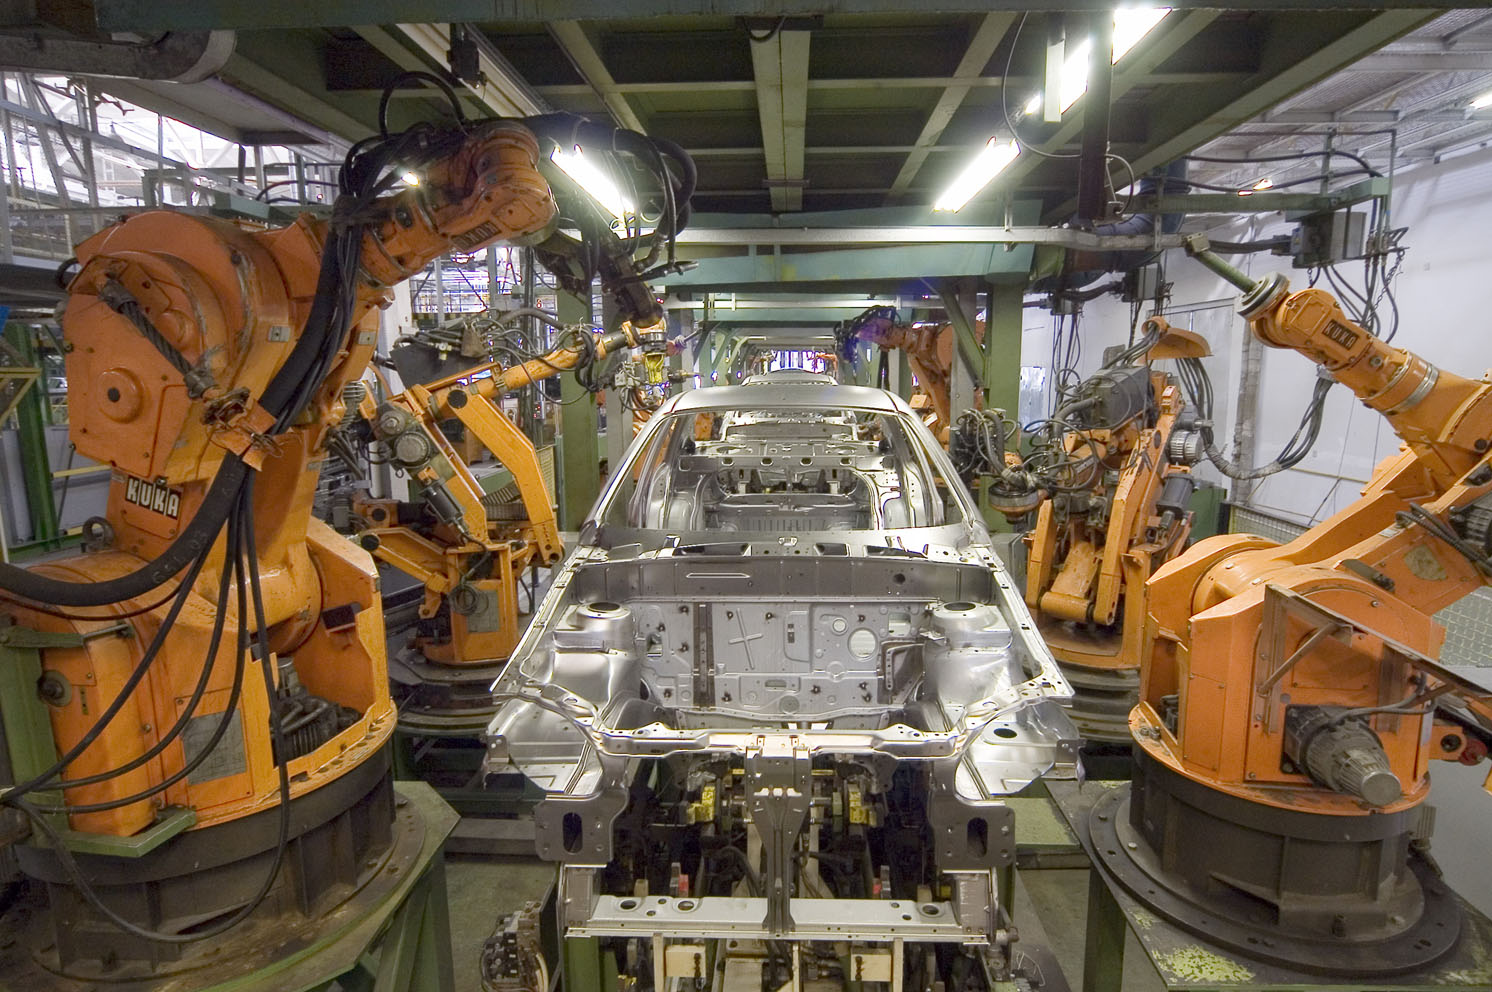
\includegraphics[width=\textwidth]{KUKA_Industrial_Robots_IR_wikimedia.jpg}
\end{center}
\caption{Des robots sur une chaîne de montage dans une usine de voitures.
 Source: https://commons.wikimedia.org/wiki/File:AKUKA\_Industrial\_Robots\_IR.jpg by Mixabest (Own work). CC BY-SA 3.0 (http://creativecommons.org/licenses/by-sa/3.0) or GFDL (http://www.gnu.org/copyleft/fdl.html), via Wikimedia Commons.}\label{fig.assemblyline}
\end{figure}

On pourrait arguer qu'il s'agit en réalité d'automates et non de robots. Cependant, les automates d'aujourd'hui s'appuient souvent sur des capteurs, à tel point qu'ils peuvent être considérés comme des robots. Toutefois, leur conception est simplifiée car ils travaillent dans un environnement personnalisé auquel les humains ne sont pas autorisés à accéder pendant que le robot travaille.

Cependant, les robots d'aujourd'hui ont besoin de plus de flexibilité, par exemple, la capacité de manipuler des objets dans différentes orientations ou de reconnaître différents objets qui doivent être emballés dans le bon ordre. Le robot peut être amené à transporter des marchandises vers et depuis des entrepôts. Cela apporte une autonomie supplémentaire, mais la caractéristique de base demeure : l'environnement est plus ou moins contraint et peut être adapté au robot.

Une flexibilité supplémentaire est requise lorsque les robots industriels interagissent avec les humains, ce qui introduit des exigences de sécurité élevées, tant pour les bras robotiques que pour les robots mobiles. En particulier, la vitesse du robot doit être réduite et la conception mécanique doit garantir que les pièces mobiles ne constituent pas un danger pour l'utilisateur. L'avantage de faire travailler des humains avec des robots est que chacun peut réaliser ce qu'il fait le mieux : les robots effectuent des tâches répétitives ou dangereuses, tandis que les humains réalisent des étapes plus complexes et définissent les tâches globales du robot, car ils sont prompts à reconnaître les erreurs et les possibilités d'optimisation.

\section{Robots mobiles autonomes}
\index{robot!mobile}

De nombreux robots mobiles sont télécommandés et effectuent des tâches telles que l'inspection de canalisations, la photographie aérienne et la neutralisation de bombes, qui dépendent d'un opérateur contrôlant l'appareil. Ces robots ne sont pas autonomes ; ils utilisent leurs capteurs pour permettre à leur opérateur d'accéder à distance à des endroits dangereux, éloignés ou inaccessibles. Certains d'entre eux peuvent être semi-autonomes, réalisant des sous-tâches automatiquement. Le pilote automatique d'un drone stabilise le vol tandis que l'homme choisit la trajectoire de vol. Un robot dans une canalisation peut contrôler son mouvement à l'intérieur de la canalisation pendant que l'homme recherche les défauts qui doivent être réparés. Les robots mobiles entièrement autonomes ne dépendent pas d'un opérateur, mais prennent des décisions par eux-mêmes et exécutent des tâches telles que le transport de matériaux tout en naviguant sur un terrain incertain (murs et portes dans les bâtiments, intersections dans les rues) et dans un environnement en constante évolution (personnes marchant autour, voitures circulant dans les rues).

Les premiers robots mobiles ont été conçus pour des environnements simples, par exemple des robots qui nettoyaient les piscines ou des tondeuses à gazon robotisées. Aujourd'hui, les aspirateurs robotisés sont largement répandus, car il s'est avéré possible de construire des robots à prix raisonnable capables de naviguer dans un environnement intérieur encombré d'obstacles.

De nombreux robots mobiles autonomes sont conçus pour aider les professionnels travaillant dans des environnements structurés tels que les entrepôts. Un exemple intéressant est un robot pour désherber les champs (Fig.~\ref{fig.agri_robot}). Cet environnement est partiellement structuré, mais une détection avancée est nécessaire pour effectuer les tâches d'identification et d'enlèvement des mauvaises herbes. Même dans les usines très structurées, les robots partagent l'environnement avec les humains et leur détection doit donc être extrêmement fiable.

\begin{figure}
\begin{center}
\includegraphics[width=0.8\textwidth]{ecorobotix.jpg}
\end{center}
\caption{Robot mobile autonome désherbant un champ (avec l'autorisation d'Ecorobotix)}
\label{fig.agri_robot}
\end{figure}

Le robot mobile autonome qui fait le plus parler de lui ces derniers temps est sans doute la voiture à conduite autonome. Ces dernières sont extrêmement difficiles à développer en raison de l'environnement incertain très complexe du trafic motorisé et des exigences strictes en matière de sécurité.

L'espace est un environnement encore plus difficile et dangereux. Les rovers martiens Sojourner et Curiosity sont des robots mobiles semi-autonomes. Le Sojourner a été actif pendant trois mois en 1997. Le Curiosity est actif depuis son atterrissage sur Mars en 2012 ! Bien qu'un conducteur humain sur Terre contrôle les missions (les routes à emprunter et les expériences scientifiques à mener), les rovers ont la capacité d'éviter les dangers de manière autonome.

Une grande partie de la recherche et du développement en robotique vise aujourd'hui à rendre les robots plus autonomes en améliorant les capteurs et en permettant un contrôle plus intelligent du robot. De meilleurs capteurs peuvent percevoir les détails de situations plus complexes, mais pour gérer ces situations, le contrôle du comportement du robot doit être très souple et adaptable. La vision, en particulier, est un domaine de recherche très actif car les caméras sont bon marché et les informations qu'elles peuvent acquérir sont très riches. Des efforts sont faits pour rendre les systèmes plus flexibles, afin qu'ils puissent apprendre d'un humain ou s'adapter à de nouvelles situations. Un autre domaine de recherche actif concerne l'interaction entre les humains et les robots. Cette interaction implique à la fois la détection et l'intelligence, mais elle doit également tenir compte de la psychologie et de la sociologie des interactions.

\section{Robots humanoïdes}\index{robot!humanoid}

La science-fiction et les médias de masse aiment représenter les robots sous une forme humanoïde. Nous connaissons tous R2-D2 et 3-CPO, les personnages robotiques des films de la Guerre des étoiles, mais le concept est très ancien. Au XVIIIe siècle, un groupe d'horlogers suisses - Pierre et Henri-Louis Jaquet-Droz et Jean-Fr'{e}d'{e}ric Leschot - ont construit des automates humanoïdes pour démontrer leurs compétences mécaniques et faire la publicité de leurs montres. Aujourd'hui, de nombreuses entreprises construisent des robots humanoïdes pour des raisons similaires.

Les robots humanoïdes sont une forme de robot mobile autonome doté d'une conception mécanique extrêmement complexe pour le mouvement des bras et la locomotion par les jambes. Les robots humanoïdes sont utilisés pour la recherche sur la mécanique de la marche et sur l'interaction homme-machine. Des robots humanoïdes ont été proposés pour assurer les services et la maintenance dans une maison ou une station spatiale. Ils sont envisagés pour fournir des soins aux personnes âgées qui pourraient se sentir anxieuses en présence d'une machine qui n'a pas l'air humaine. D'autre part, les robots qui ressemblent beaucoup aux humains peuvent générer de la répulsion, un phénomène appelé la \emph{uncanny valley}.

Les robots humanoïdes peuvent être très difficiles à concevoir et à contrôler. Ils sont coûteux à construire et comportent de multiples articulations qui peuvent se déplacer de nombreuses façons différentes. Les robots qui utilisent des roues ou des chenilles sont préférés pour la plupart des applications car ils sont plus simples, moins chers et plus robustes.

\section{Robots éducatifs}\label{s.educational}
\index{robot!éducatif}

Les progrès de l'électronique et de la mécanique ont permis de construire des robots relativement peu coûteux. Les robots éducatifs sont largement utilisés dans les écoles, tant en classe que dans le cadre d'activités extrascolaires. Le grand nombre de robots éducatifs ne permet pas d'en donner un aperçu complet. Nous donnons ici quelques exemples représentatifs des robots couramment utilisés dans l'enseignement.

\medskip

\noindent\textbf{Robots mobiles préassemblés}

De nombreux robots éducatifs sont conçus comme des robots mobiles préassemblés. La Fig.~\ref{fig.thymio} montre le robot Thymio de Mobsya et la Fig.~\ref{fig.dash} montre le robot Dash de Wonder Workshop. Ces robots sont relativement peu coûteux, robustes et contiennent un grand nombre de capteurs et de composants de sortie tels que des lumières. Un avantage important de ces robots est que vous pouvez mettre en œuvre des algorithmes robotiques "prêts à l'emploi", sans investir des heures dans la conception et la construction mécanique. Cependant, les robots pré-assemblés ne peuvent pas être modifiés, bien que beaucoup d'entre eux permettent de construire des extensions en utilisant, par exemple, des composants \lego{}.

\begin{figure}
\begin{minipage}{.45\textwidth}
\begin{center}
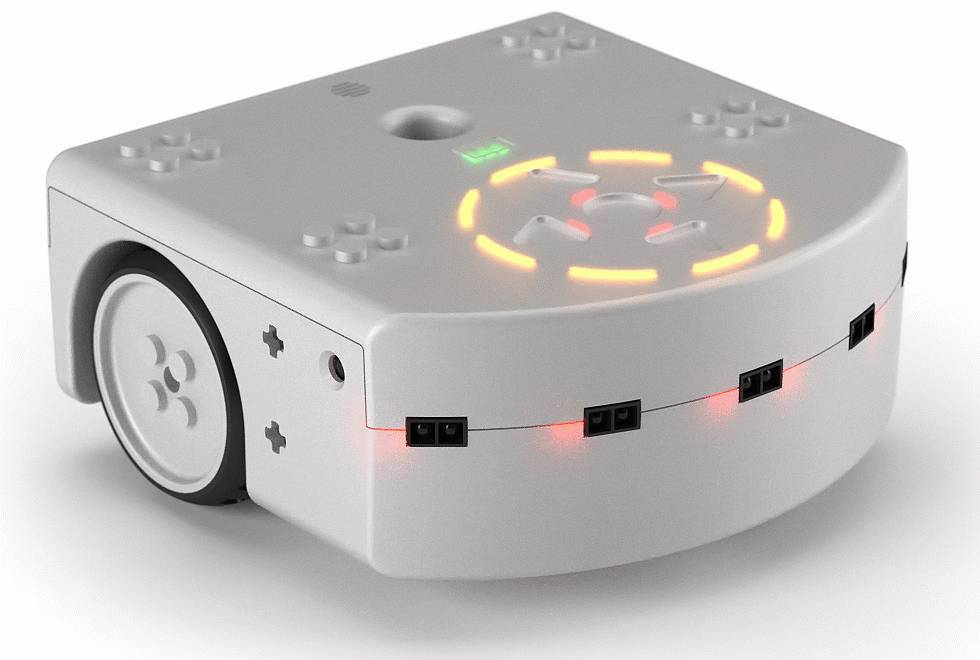
\includegraphics[width=.45\textwidth]{thymio}
\caption{Le robot Thymio. Source : \protect\url{https://www.thymio.org/en:mediakit} avec l'autorisation de \'{E}cole Polytechnique F\'{e}d\'{e}rale de Lausanne and \'{E}cole Cantonale d'Art de Lausanne.}\label{fig.thymio}
\end{center}
\end{minipage}
\hspace{\fill}
\begin{minipage}{.45\textwidth}
\begin{center}
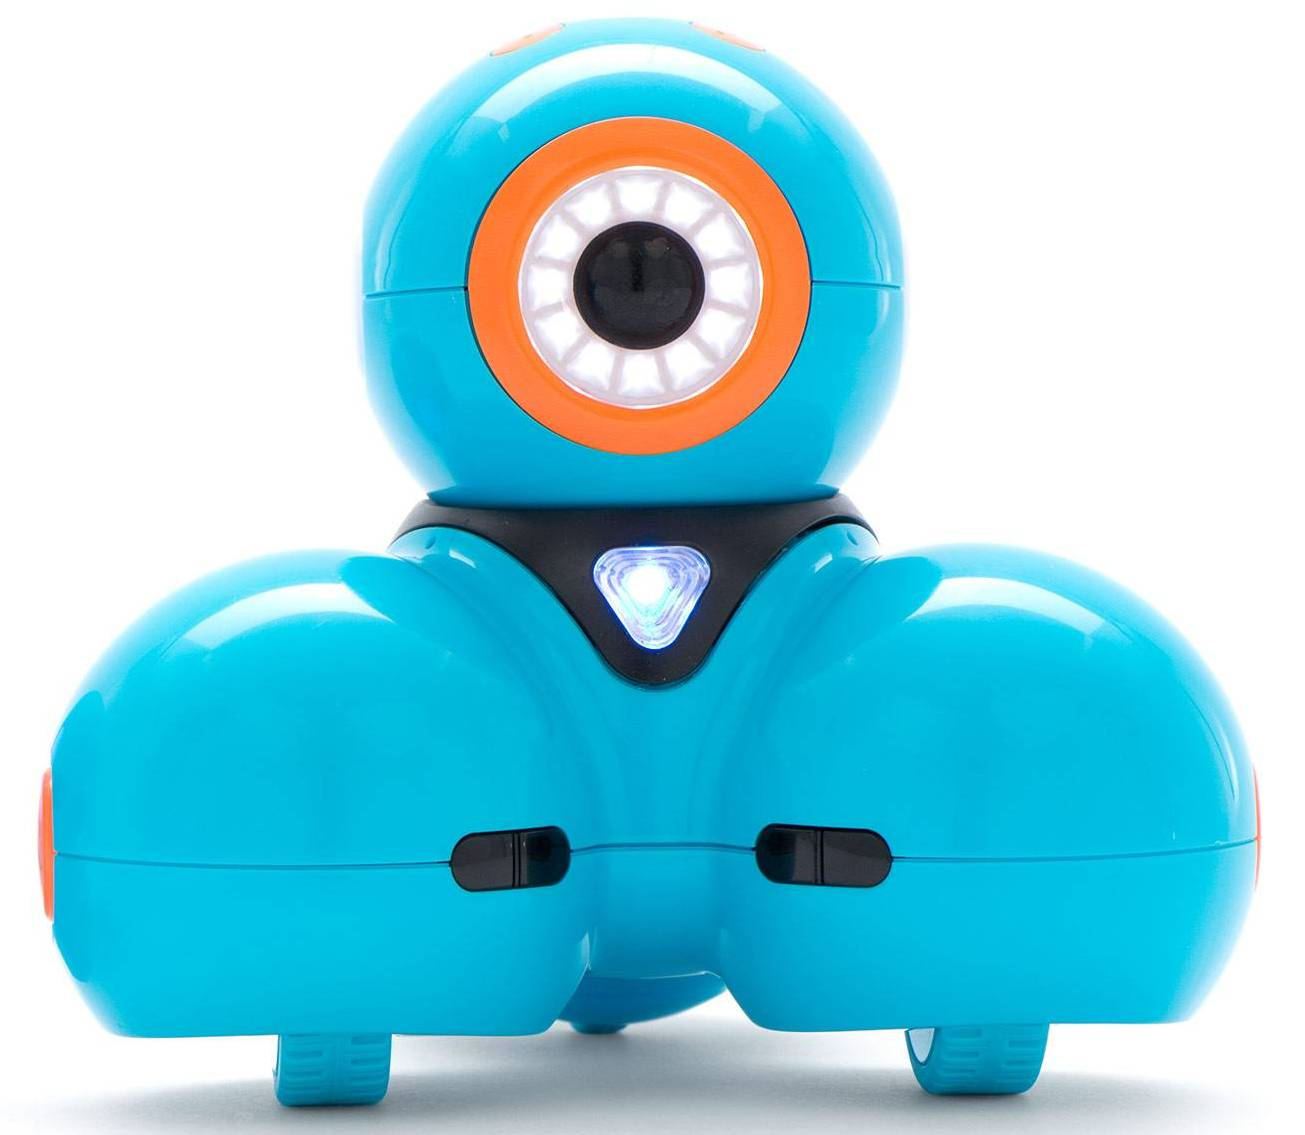
\includegraphics[width=.45\textwidth]{dash}
\caption{Robot Dash. Source : \protect\url{https://www.makewonder.com/mediakit} avec l'autorisation de Wonder Workshop.}\label{fig.dash}
\end{center}
\end{minipage}
\end{figure}

\noindent\textbf{Kits de robotique}

Les kits robotiques \lego{} Mindstorms (Fig. ~\ref{fig.lego}) ont été lancés en 1998. \footnote{La figure montre la dernière version appelée \emph{EV3} introduite en 2014.} Un kit se compose de briques \lego{} standard et d'autres éléments de construction, ainsi que de moteurs et de capteurs, et d'une brique programmable qui contient l'ordinateur qui contrôle les composants du robot. L'avantage des kits robotiques est qu'ils sont flexibles : vous pouvez concevoir et construire un robot pour effectuer une tâche spécifique, en n'étant limité que par votre imagination. Un kit de robotique peut également être utilisé pour enseigner la conception mécanique aux étudiants. Les inconvénients des kits robotiques sont qu'ils sont plus coûteux que les simples robots préassemblés et que l'exploration des algorithmes robotiques dépend de la capacité de chacun à mettre en œuvre avec succès une conception mécanique robuste.

Une tendance récente consiste à remplacer les collections fixes de briques par des pièces construites par des imprimantes 3D. Le bras robotique Poppy Ergo Jr (Fig.~\ref{fig.poppy}) en est un exemple. L'utilisation de pièces imprimées en 3D permet une plus grande flexibilité dans la création de la structure mécanique et une plus grande robustesse, mais nécessite l'accès à une imprimante 3D. 

\begin{figure}
\begin{minipage}{.45\textwidth}
\begin{center}
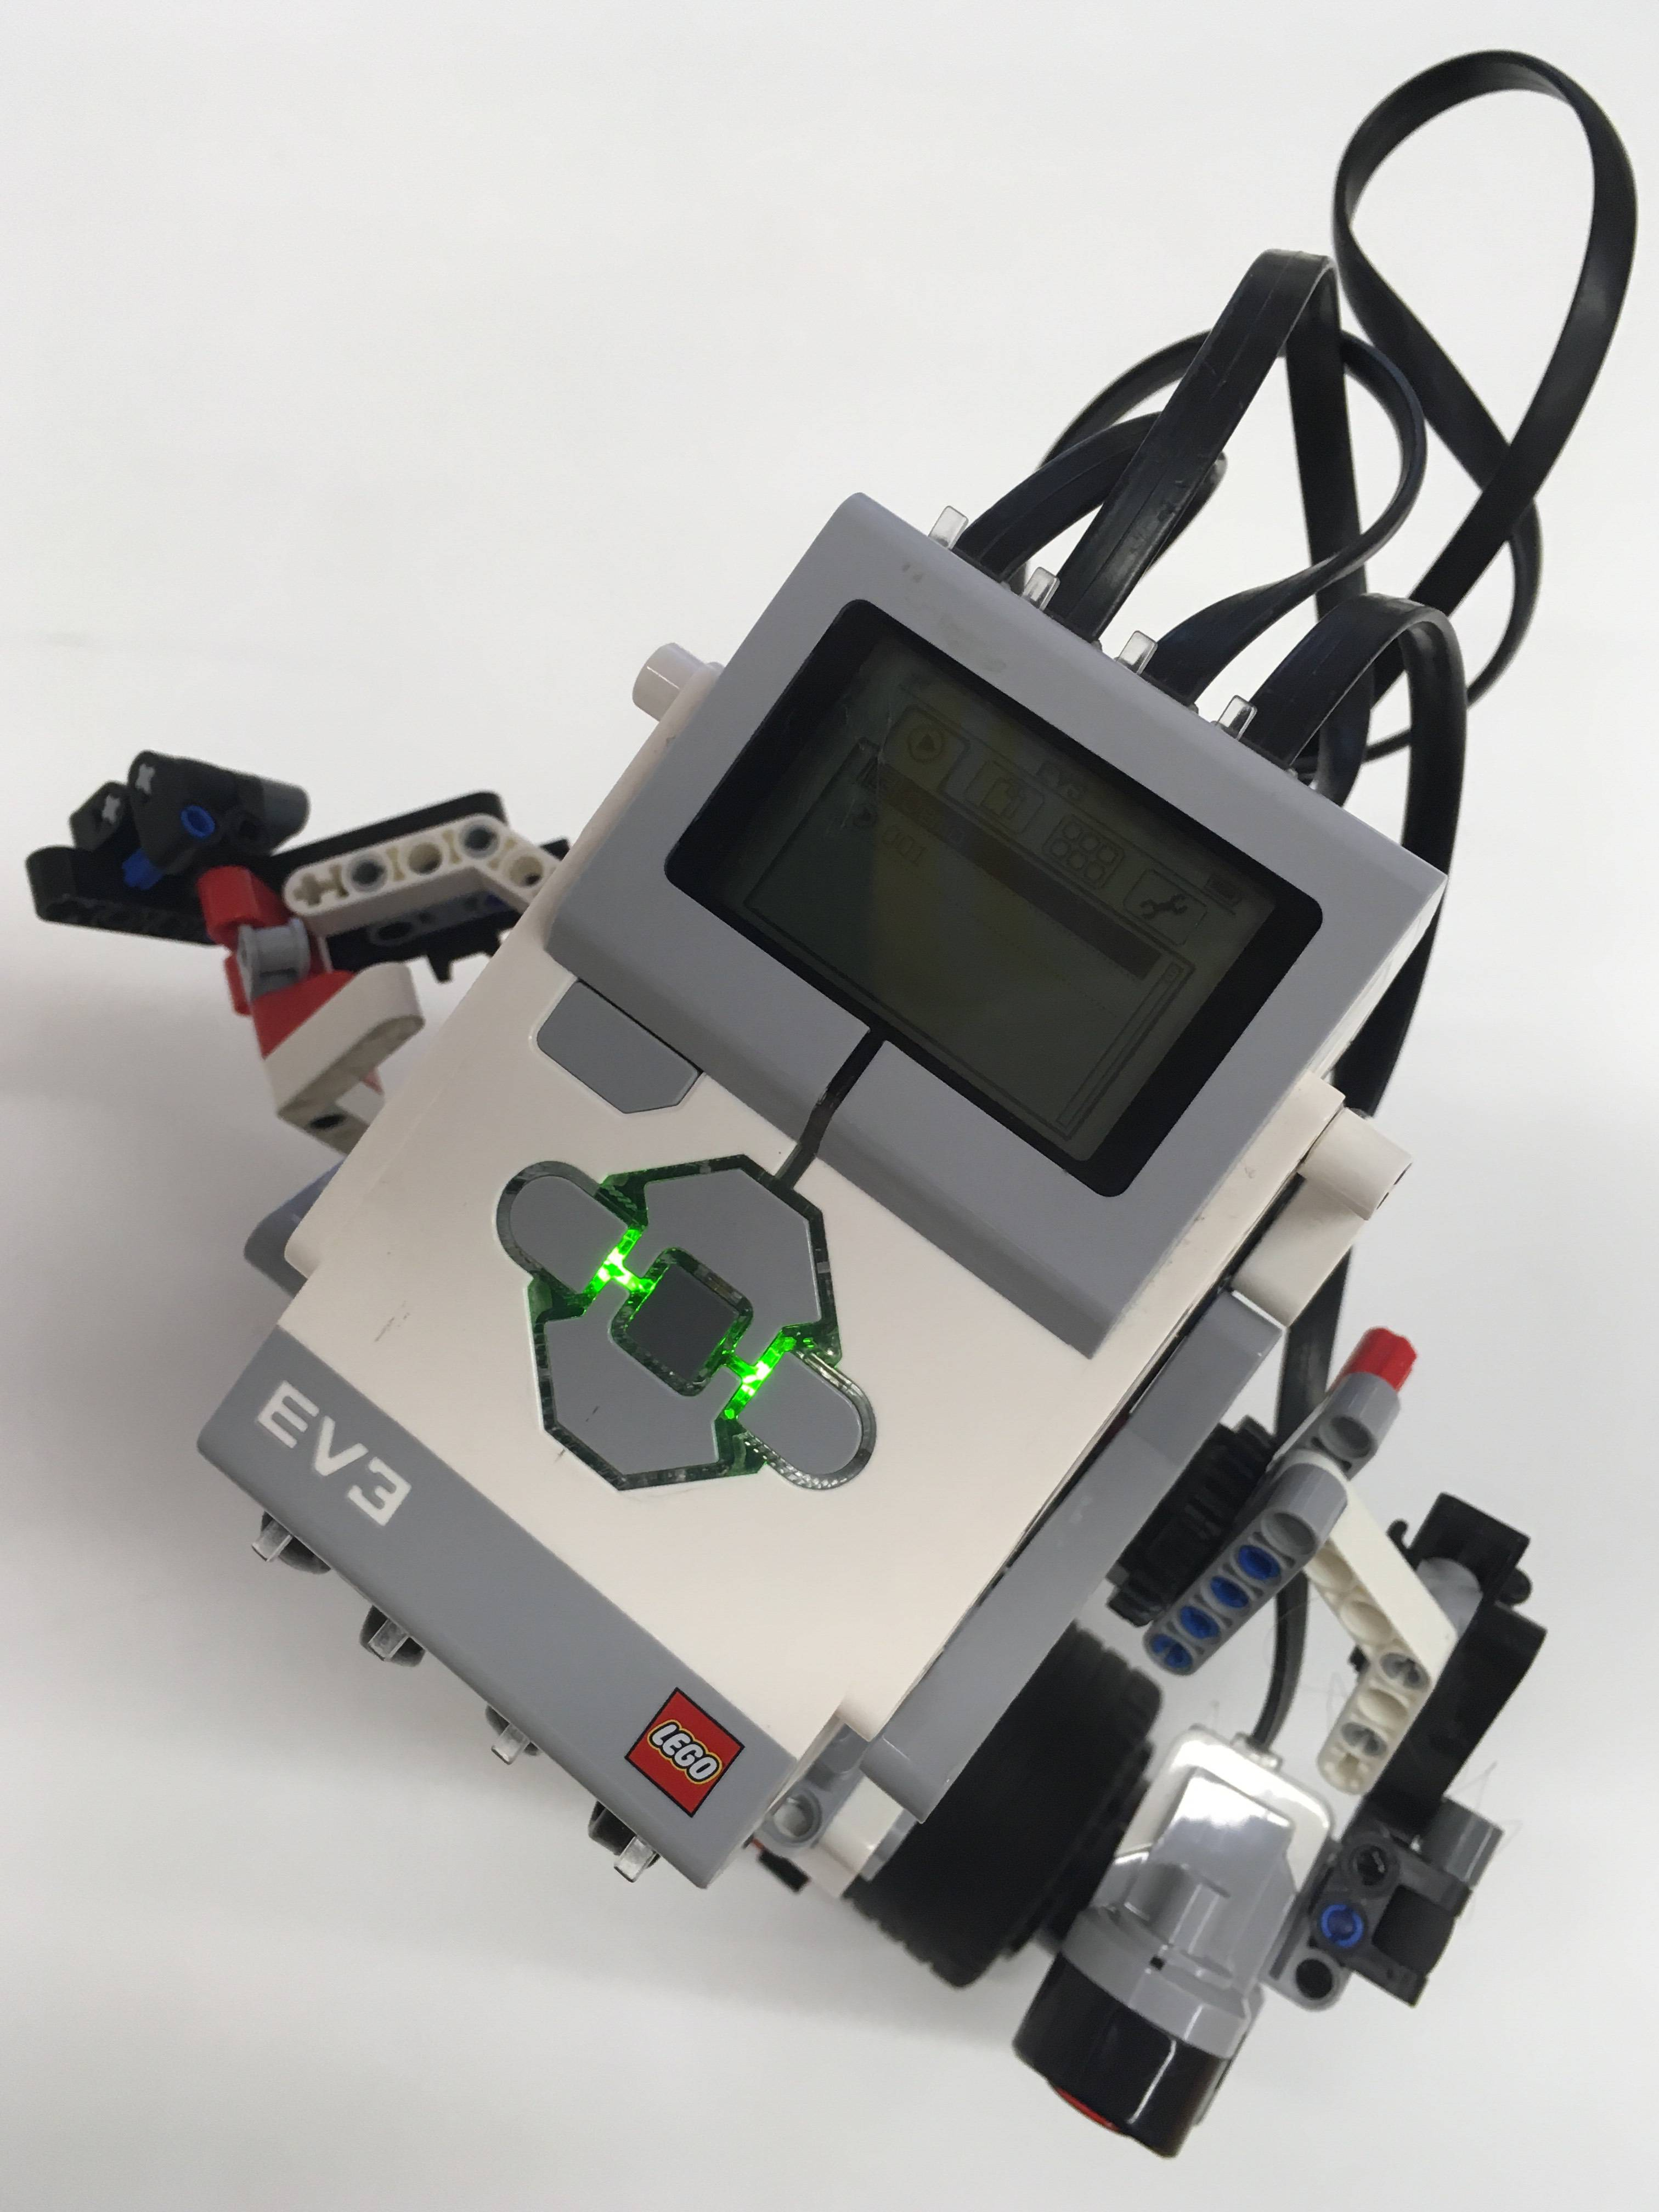
\includegraphics[width=.4\textwidth]{lego}
\end{center}
\caption{\lego{} Mindstorms EV3 (avec l'aimable autorisation d'Adi Shmorak, Intelitek)}
\label{fig.lego}
\end{minipage}
\hspace{\fill}
\begin{minipage}{.45\textwidth}
\begin{center}
\includegraphics[width=.55\textwidth]{ErgoJr.jpg}
\end{center}
\caption{Bras robotisés Poppy Ergo Jr (avec l'aimable autorisation du Poppy Project)}
\label{fig.poppy}
\end{minipage}
\end{figure}


\noindent\textbf{Bras robotiques}

Pour agir sur son environnement, le robot a besoin d'un \emph{actuateur} qui est un composant d'un robot qui affecte l'environnement. De nombreux robots, en particulier les bras robotisés utilisés dans l'industrie, agissent sur l'environnement par le biais d'effecteurs finaux, généralement des pinces ou des outils similaires (Figs.~\ref{fig.assemblyline}, \ref{fig.sortballs}, \ref{fig.robots-pulling}). Les actionneurs des robots mobiles sont les moteurs qui font bouger le robot, ainsi que des composants tels que la pompe à vide d'un aspirateur.

Les robots éducatifs sont généralement des robots mobiles dont les seuls actionneurs sont ses moteurs et des dispositifs d'affichage tels que des lumières, des sons ou un écran. Les effecteurs peuvent être construits avec des kits de robotique ou en utilisant des composants supplémentaires avec des robots pré-assemblés, bien que des bras robotiques éducatifs existent (Fig.~ref{fig.poppy}). La manipulation d'objets introduit une certaine complexité dans la conception ; cependant, les algorithmes des effecteurs finaux étant similaires à ceux des robots mobiles simples, la plupart des activités de ce livre supposeront uniquement que votre robot dispose de moteurs et de dispositifs d'affichage.

\medskip

\noindent\textbf{Environnements de développement de logiciels}

Chaque système de robotique éducative comprend un \emph{environnement de développement logiciel}\index{environnement de développement logiciel}. Le langage de programmation peut être une version d'un langage de programmation standard comme Java ou Python. La programmation est simplifiée si un langage à base de blocs est utilisé, généralement un langage basé sur Scratch ou Blockly (Fig.~\ref{fig.ide-blocks}).

\begin{figure}
\begin{center}
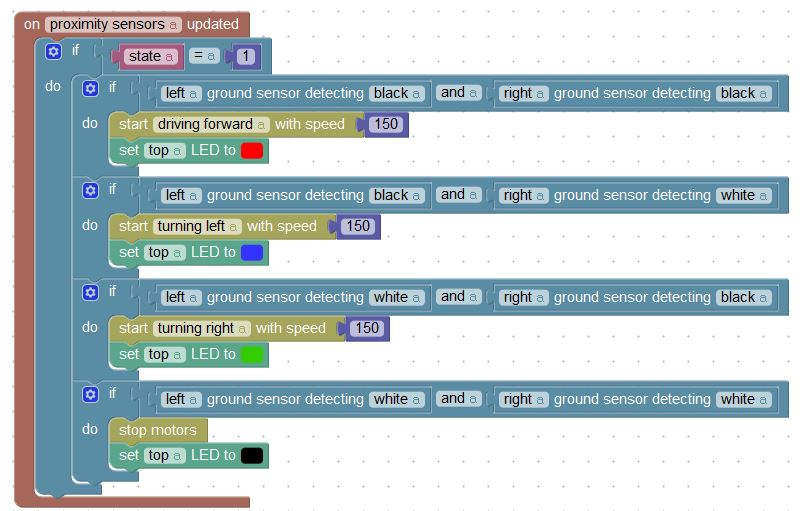
\includegraphics[width=.7\textwidth]{blockly}
\end{center}
\caption{Logiciel blockly pour le robot Thymio}\label{fig.ide-blocks}
\end{figure}

Pour simplifier davantage la programmation d'un robot par de jeunes étudiants, une notation de programmation entièrement graphique peut être utilisée. Les figures~\ref{fig.ide-thymio} montrent le VPL (Visual Programming Language), un environnement logiciel graphique pour le robot Thymio. Il utilise des paires événement-action : lorsque l'événement représenté par le bloc de gauche se produit, les actions des blocs suivants sont exécutées.

\begin{figure}
\begin{center}
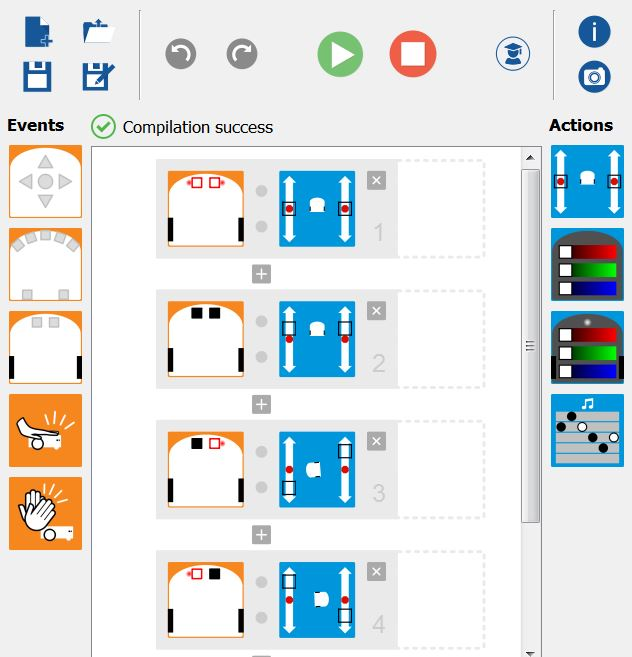
\includegraphics[width=.7\textwidth]{vpl}
\end{center}
\caption{Logiciel VPL pour le robot Thymio}\label{fig.ide-thymio}
\end{figure}

La figure~\ref{fig.ide-dash} montre l'environnement logiciel graphique pour le robot Dash. Il utilise également des événements et des actions, où les actions sont représentées par des nœuds et les événements par des flèches entre les nœuds.

\begin{figure}
\begin{center}
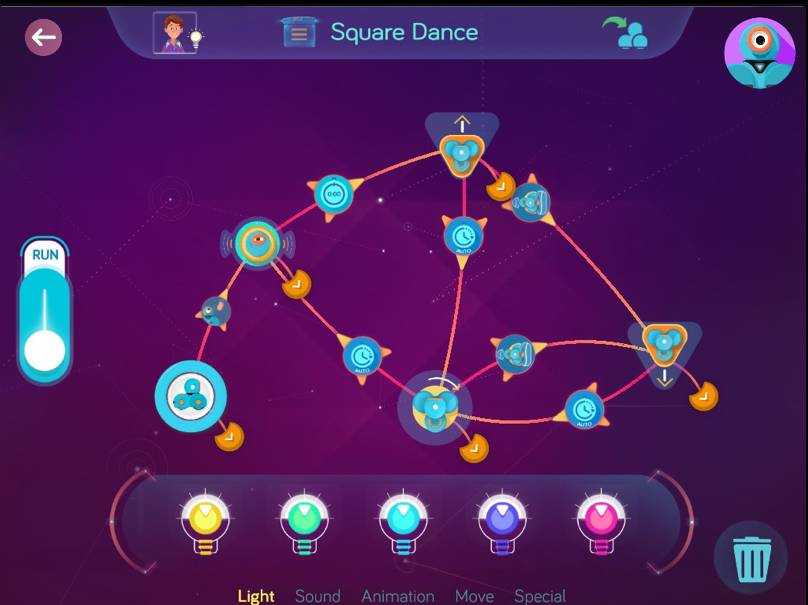
\includegraphics[width=.8\textwidth]{wonder}
\end{center}
\caption{Les logiciels Wonder pour le robot Dash (Avec l'aimable autorisation de Wonder Workshop)}\label{fig.ide-dash}
\end{figure}

\section{Le robot générique}\label{s.generic}

\index{robot!generic}
Cette section présente la description d'un robot générique que nous utilisons pour présenter les algorithmes de robotique. Les capacités du robot générique sont similaires à celles des robots éducatifs, mais celui que vous utiliserez n'aura peut-être pas toutes les capacités supposées dans les présentations ; vous devrez donc improviser. Vous ne comprendrez peut-être pas encore tous les termes de la description suivante, mais il est important que la spécification soit formalisée. Des détails supplémentaires seront donnés dans les chapitres suivants.

\subsection{Direction différentielle}

Le robot est un petit véhicule autonome doté d'une \emph{motorisation différentielle},\index{motorisation différentielle}, ce qui signifie qu'il possède deux roues entraînées par des moteurs indépendants (Fig.~\ref{fig.differential}). Pour faire bouger le robot, réglez la puissance du moteur sur une valeur comprise entre $-100$ (pleine puissance en arrière), $0$ (arrêt) et $100$ (pleine puissance en avant). Il n'y a pas de relation prédéfinie entre la puissance du moteur et la vitesse du robot. Le moteur peut être relié aux roues par différents rapports d'engrenage, le type de pneus sur les roues affecte leur traction, et un terrain sablonneux ou boueux peut faire glisser les roues.

\begin{figure}
\begin{center}
\begin{tikzpicture}[scale=1.2]
\pic[scale=1.5] at (0,0) { robot };
\draw[densely dotted,thick] (12mm,0) circle[radius=6pt];
\draw[->] (16mm,10mm) node[right] {\p{support (sur la partie inférieure du robot))}} -- (13mm,3mm);
\draw[->,thick] (20mm,0) -- node[below] {\p{avant} } +(18mm,0);
\draw[raxis] (0,0) -- (0,15mm);
\draw[raxis] (0,0) -- (0,-15mm);
\draw[raxis] (0,0) -- (11pt,0);
\draw[raxis] (0,0) -- (-11pt,0);
\end{tikzpicture}
\end{center}
\caption{Robot à entraînement différentiel\label{fig.differential}}
\end{figure}

La figure~\ref{fig.differential} montre une vue du robot depuis le haut. L'avant du robot est la courbe vers la droite, qui correspond également à la direction avant du mouvement du robot. Les roues (rectangles noirs) se trouvent sur les côtés gauche et droit de l'arrière du corps du robot. Le point est le point de l'essieu situé à mi-chemin entre les roues. Lorsque le robot tourne, il tourne autour d'un axe vertical à ce point. Pour la stabilité, vers l'avant du robot se trouve un support ou une roue non motrice.

\begin{quote}
\begin{center}
\textbf{Dessin mécanique}
\end{center}
Une ligne brisée est la notation standard en ingénierie mécanique pour l'axe de symétrie d'un composant tel qu'une roue. Lorsque la vue latérale d'une roue est affichée, l'intersection des deux axes de symétrie indique l'axe de rotation qui est perpendiculaire au plan de la page. Pour ne pas encombrer les diagrammes, nous simplifions la notation en ne montrant que des lignes brisées pour un \emph{axe de rotation} d'un composant tel qu'une roue. En outre, l'intersection désignant un axe perpendiculaire est généralement abrégée en croix, éventuellement contenue dans la roue ou son essieu.
\end{quote}

L'entraînement différentiel présente plusieurs avantages : il est simple puisqu'il ne comporte que deux moteurs sans composants supplémentaires pour la direction et il permet au robot de tourner sur place. Dans une voiture, deux roues sont entraînées ensemble (ou quatre roues sont entraînées par paires) et il existe un mécanisme complexe distinct pour la direction appelé \emph{Direction d'Ackermann}\index{Direction d'Ackermann}. Étant donné qu'une voiture ne peut pas tourner sur place, les conducteurs doivent effectuer des manœuvres compliquées telles que le stationnement parallèle ; les conducteurs humains apprennent facilement à le faire, mais de telles manœuvres sont difficiles pour un système autonome. Un robot autonome doit effectuer des manœuvres complexes avec des mouvements très simples, c'est pourquoi l'entraînement différentiel est la configuration préférée : il peut facilement tourner vers n'importe quel cap et se déplacer ensuite dans cette direction.

Le principal inconvénient d'un système d'entraînement différentiel est qu'il nécessite un troisième point de contact avec le sol, contrairement à une voiture qui a déjà quatre roues pour la soutenir et qui peut donc se déplacer facilement sur un terrain difficile. Un autre inconvénient est qu'il ne peut pas se déplacer latéralement sans tourner. Il existe des configurations qui permettent à un robot de se déplacer latéralement (Sect.~\ref{s.holonomic}), mais elles sont complexes et coûteuses. L'entraînement différentiel est également utilisé dans les véhicules à chenilles tels que les engins de terrassement et les chars militaires. Ces véhicules peuvent manœuvrer sur des terrains extrêmement accidentés, mais les chenilles produisent beaucoup de friction et les mouvements sont lents et peu précis.

\begin{quote}
\begin{center}
\textbf{Réglage de la puissance ou de la vitesse}
\end{center}
La puissance fournie par un moteur est régulée par un \emph{throttle}, comme une pédale dans une voiture ou des leviers dans un avion ou un bateau. Les moteurs électriques utilisés dans les robots mobiles sont contrôlés en modifiant la tension appliquée aux moteurs à l'aide d'une technique appelée \emph{modulation de largeur d'impulsion}. Dans de nombreux robots éducatifs, des algorithmes de contrôle, tels que ceux décrits dans le Chap.~\ref{ch.control}, sont utilisés pour garantir que les moteurs tournent à une \emph{vitesse cible} spécifiée. Étant donné que nous nous intéressons aux concepts et aux algorithmes de conception de robots, nous exprimerons les algorithmes en termes de fourniture de puissance et traiterons séparément le contrôle de la vitesse.
\end{quote}

\subsection{Capteurs de proximité}

Le robot dispose de \emph{capteurs de proximité horizontaux}\index{capteurs!de proximité} qui peuvent détecter un objet à proximité du robot. Il existe de nombreuses technologies pouvant être utilisées pour construire ces capteurs, comme l'infrarouge, le laser, les ultrasons ; le robot générique représente les robots qui utilisent l'une de ces technologies. Nous spécifions que les capteurs doivent avoir les capacités suivantes : Un capteur de proximité horizontal peut mesurer la distance (en centimètres) entre le robot et un objet et l'angle (en degrés) entre l'avant du robot et l'objet. La figure~\ref{fig.generic-sensor} montre un objet situé à $3\,$ cm du centre du robot à un angle de $45^{\circ}$ par rapport à la direction vers laquelle pointe le robot.\footnote{Voir Annexe~\ref{ch.units} sur les conventions de mesure des angles.}

\begin{figure}
\begin{minipage}{.45\textwidth}
\begin{tikzpicture}
\pic[scale=1.2] at (0,0) { robot };
\draw[->] (0,0) -- node[sloped,above] {$3\,$cm} (45:2.5cm) node[above right=-4pt] {$\bullet$};
\draw[dashed] (0,0) node[above,xshift=20pt] {$45^{\circ}$}-- (2.5,0);
\draw (10pt,0) arc [start angle=0, end angle=45, radius=10pt];
\fill[gray] (0,0) circle[radius=4pt];
\end{tikzpicture}
\caption{Robot avec capteur rotatif (point gris)}
\label{fig.generic-sensor}
\end{minipage}
\hspace{\fill}
\begin{minipage}{.45\textwidth}
\begin{tikzpicture}
\pic[scale=1.2] at (0,0) { robot2 };
\end{tikzpicture}
\caption{Robot avec deux capteurs de sol sur la partie inférieure du robot (rectangles gris)}
\label{fig.generic-ground}
\end{minipage}
\end{figure}


En pratique, un robot éducatif dispose d'un petit nombre de capteurs et ne peut donc pas détecter les objets dans toutes les directions. De plus, les capteurs bon marché ne seront pas en mesure de détecter des objets très éloignés et leurs mesures ne seront pas précises. Les mesures seront également affectées par des facteurs environnementaux tels que le type d'objet, la lumière ambiante, etc. Pour simplifier nos algorithmes, nous ne supposons pas de limites prédéfinies, mais lorsque vous implémenterez les algorithmes, vous devrez tenir compte de ces limites.

\subsection{Capteurs de sol}

\emph{Capteurs de sol}\index{capteur!sol} sont montés sur la partie inférieure du robot. Étant donné que ces capteurs sont très proches du sol, la distance ou l'angle n'ont aucune signification ; au lieu de cela, le capteur mesure la luminosité de la lumière réfléchie par le sol dans des valeurs arbitraires comprises entre $0$ (totalement sombre) et $100$ (totalement clair). Le robot générique possède deux capteurs de sol montés à l'avant du robot (Fig.~ref{fig.generic-ground}), bien que nous présentions parfois des algorithmes qui n'utilisent qu'un seul capteur. La figure montre une vue de dessus du robot, bien que les capteurs de sol se trouvent sur la partie inférieure du robot.

\subsection{Ordinateur embarqué}\label{s.embedded}

Le robot est équipé d'un \emph{ordinateur intégré} (Fig.~\ref{fig.computer}). La spécification précise de l'ordinateur n'est pas importante mais nous supposons certaines capacités. L'ordinateur peut lire les valeurs des capteurs et régler la puissance des moteurs. Il est possible d'afficher des informations sur un petit écran ou d'utiliser des lumières colorées. Les signaux et les données peuvent être introduits dans l'ordinateur à l'aide de boutons, d'un clavier ou d'une télécommande.

\begin{figure}
\begin{center}
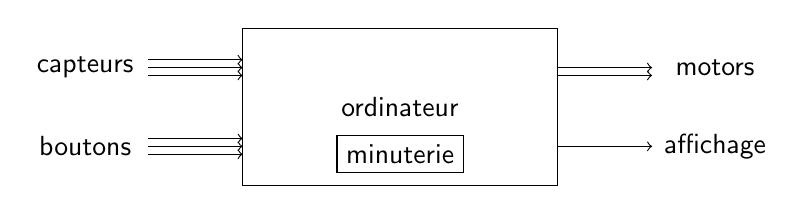
\begin{tikzpicture}
\node[draw,rectangle,minimum width=4cm,minimum height=2cm] at (0,0) {\textsf{ordinateur}};
\node[draw,rectangle] at (0,-.6) {\textsf{minuterie}};
\node at (-4,.5) {\textsf{capteurs}};
\node at (-4,-.5) {\textsf{boutons}};
\draw[->] (-3.2,.4) -- (-2,.4);
\draw[->] (-3.2,.5) -- (-2,.5);
\draw[->] (-3.2,.6) -- (-2,.6);
\draw[->] (-3.2,-.4) -- (-2,-.4);
\draw[->] (-3.2,-.5) -- (-2,-.5);
\draw[->] (-3.2,-.6) -- (-2,-.6);
\node at (4,.5) {\textsf{motors}};
\node at (4,-.5) {\textsf{affichage}};
\draw[->] (2,.4) -- (3.2,.4);
\draw[->] (2,.5) -- (3.2,.5);
\draw[->] (2,-.5) -- (3.2,-.5);
\end{tikzpicture}
\caption{Ordinateur embarqué}\label{fig.computer}
\end{center}
\end{figure}

Les données sont introduites dans l'ordinateur par des \emph{événements}, par exemple en touchant un bouton. L'occurrence d'un événement entraîne l'exécution d'une procédure appelée \emph{event handler}\index{event handler}. L'événement peut être détecté par le matériel, auquel cas le terme \emph{interruption} est utilisé, ou il peut être détecté par le logiciel, généralement, par \emph{polling}, où le système d'exploitation vérifie les événements à des intervalles prédéfinis. Lorsque le gestionnaire d'événements se termine, le calcul précédent est relancé.

Les gestionnaires d'événements sont différents des programmes séquentiels qui ont une instruction initiale qui entre des données et une instruction finale qui affiche la sortie, car les gestionnaires d'événements sont exécutés en réponse à des événements imprévisibles. Le traitement des événements est utilisé pour mettre en œuvre des interfaces utilisateur graphiques sur les ordinateurs et les smartphones : lorsque vous cliquez sur une icône ou que vous la touchez, un gestionnaire d'événements est exécuté. Sur un robot, un événement peut être une entrée discrète, comme le fait de toucher une touche. Les événements peuvent également se produire lorsqu'une valeur continue, telle que la valeur lue par un capteur, est supérieure ou inférieure à une valeur prédéfinie appelée \emph{threshold}\index{threshold}.

L'ordinateur comprend un \emph{timer}\index{timer} qui fonctionne comme un chronomètre sur un smartphone. Un chronomètre est une variable qui est \emph{set} sur une période de temps, par exemple, $0,5$ seconde, qui est représentée par un nombre entier de millisecondes ou de microsecondes ($0,5$ seconde est $500$ millisecondes). L'horloge matérielle de l'ordinateur provoque une interruption à intervalles fixes et le système d'exploitation décrémente la valeur du minuteur. Lorsque sa valeur atteint zéro, on dit que la minuterie a \emph{expiré} ; une interruption se produit.

Les minuteurs sont utilisés pour mettre en œuvre des événements répétés, comme l'allumage et l'extinction d'une lumière. Ils sont également utilisés pour le \emph{polling}\index{polling}, une alternative aux gestionnaires d'événements : au lieu d'effectuer un calcul lorsqu'un événement se produit, les capteurs sont lus et stockés périodiquement. Plus précisément, le polling se produit comme un gestionnaire d'événements lorsqu'un timer expire, mais la conception d'un logiciel utilisant le polling peut être très différente de celle d'un logiciel basé sur des événements.

\section{Le formalisme algorithmique}\label{s.alg-formalism}

Les algorithmes mis en œuvre sous forme de programmes informatiques sont utilisés par l'ordinateur embarqué pour contrôler le comportement du robot. Nous ne donnons pas de programmes dans un langage de programmation spécifique ; au lieu de cela, les algorithmes sont présentés dans un \emph{pseudocode},\index{pseudocode} un format structuré utilisant une combinaison de langage naturel, de mathématiques et de structures de programmation. L'algorithme~\ref{alg.integer-mult} est un algorithme simple de multiplication d'entiers par addition répétée. L'entrée de l'algorithme est une paire d'entiers et la sortie est le produit des deux valeurs d'entrée. L'algorithme déclare trois variables entières : \p{x}, \p{a}, \p{b}. Il y a cinq instructions dans la partie exécutable. L'indentation est utilisée (comme dans le langage de programmation Python) pour indiquer la portée de la boucle. Une flèche est utilisée pour l'affectation, afin que les symboles familiers $=$ et $\neq$ puissent être utilisés pour l'égalité et l'inégalité dans les formules mathématiques.\footnote{Beaucoup de langages de programmation utilisent \texttt{=} pour l'affectation, puis \texttt{==} pour l'égalité et \texttt{!=} pour l'inégalité. Cela prête à confusion car l'égalité $x=y$ est symétrique, mais l'affectation ne l'est pas \texttt{x=x+1}. Nous préférons conserver la notation mathématique.}

\begin{figure}
\begin{alg}{Multiplication des nombres entiers}{integer-mult}           
&\idv{}integer x \ass 0&\\
&\idv{}integer a, b&\\
\hline
\stl{}&a \ass input an integer&\\
\stl{}&b \ass input a non-negative integer&\\
\stl{}&while b $\neq$ 0&\\
\stl{}&\idc{} x \ass x $+$ a&// Add the value a to x\\
\stl{}&\idc{} b \ass b $-$ 1&// \ \ for each b\\
\end{alg}
\end{figure}

La puissance du moteur est définie à l'aide d'instructions d'affectation :
\begin{quote}
\p{left-motor-power} \ass $50$\\
\p{right-motor-power} \ass $-50$
\end{quote}

Nous avons défini nos capteurs de proximité comme renvoyant la distance à un objet détecté et son angle par rapport à la direction avant du robot, mais il sera souvent plus pratique d'utiliser des expressions en langage naturel telles que :
\begin{quote}
\p{when object detected in front}\\
\p{when object not detected in back}
\end{quote}

\section{Un aperçu du contenu du livre}\label{s.overview}

Les six premiers chapitres constituent le cœur des concepts et des algorithmes de la robotique.
\begin{description}
\item [\textbf{Chapitre \ref{ch.basic} Les robots et leurs applications}] Ce chapitre présente et classe les robots. Il précise également le robot générique et les formalismes utilisés pour présenter les algorithmes dans ce livre.
\smallskip
\item [\textbf{Chapitre \ref{ch.sensors} Capteurs}] Les robots sont plus que des appareils contrôlés à distance comme un téléviseur. Ils présentent un comportement autonome basé sur la détection d'objets dans leur environnement à l'aide de capteurs. Ce chapitre donne un aperçu des capteurs utilisés par les robots et explique les concepts de portée, de résolution, de précision et d'exactitude. Il traite également de la non-linéarité des capteurs et de la manière de la gérer.
\smallskip
\item [\textbf{Chapitre \ref{ch.reactive} Comportement réactif}] Lorsqu'un robot autonome détecte un objet dans son environnement, il réagit en modifiant son comportement. Ce chapitre présente les algorithmes robotiques dans lesquels le robot modifie directement son comportement en fonction des données fournies par ses capteurs. Les véhicules de Braitenberg sont des exemples simples mais élégants de comportement réactif. Le chapitre présente plusieurs variantes d'algorithmes de suivi de ligne.
\smallskip
\item [\textbf{Chapitre \ref{ch.fmg} Machines à états finis}] Un robot peut se trouver dans différents états, où sa réaction aux entrées provenant de ses capteurs dépend non seulement de ces valeurs mais aussi de l'état actuel. Les machines à états finis sont un formalisme permettant de décrire les états et les transitions entre eux qui dépendent de l'occurrence d'événements.
\smallskip
\item [\textbf{Chapitre \ref{ch.motion} Mouvement robotique et odométrie}] Les robots autonomes explorent leur environnement en effectuant des actions. Il ne se passe pas un jour sans qu'un rapport sur l'expérience des voitures autonomes ne soit publié. Ce chapitre passe en revue les concepts liés au mouvement (distance, temps, vitesse, accélération), puis présente l'odométrie, la méthode fondamentale qu'utilise un robot pour se déplacer d'une position à une autre. L'odométrie est sujette à des erreurs importantes et il est important de comprendre leur nature.

La deuxième partie du chapitre donne un aperçu des concepts avancés du mouvement robotique : les encodeurs de roue et les systèmes de navigation inertielle qui peuvent améliorer la précision de l'odométrie, et les degrés de liberté et l'holonomie qui affectent la planification du mouvement robotique.
\smallskip
\item [\textbf{Chapitre \ref{ch.control} Contrôle}] Un robot autonome est un système de contrôle en boucle fermée, car les entrées de ses capteurs affectent son comportement qui, à son tour, affecte ce qui est mesuré par les capteurs. Par exemple, une voiture autonome qui s'approche d'un feu de circulation peut freiner plus fort à mesure qu'elle se rapproche du feu. Ce chapitre décrit les mathématiques des systèmes de contrôle qui assurent un comportement optimal : la voiture s'arrête effectivement au feu et le freinage est progressif et doux.
\end{description}

Un robot mobile autonome doit d'une manière ou d'une autre naviguer d'une position de départ à une position d'arrivée, par exemple pour apporter des médicaments de la pharmacie d'un hôpital au patient. La navigation est un problème fondamental en robotique qui est difficile à résoudre. Les quatre chapitres suivants présentent des algorithmes de navigation dans divers contextes.
\begin{description}
\item [\textbf{Chapitre \ref{ch.obstacle} Navigation locale : évitement d'obstacles}] L'exigence la plus fondamentale pour un robot mobile est qu'il ne s'écrase pas sur les murs, les personnes et autres obstacles. C'est ce qu'on appelle la navigation \emph{locale}, car elle concerne le voisinage immédiat du robot et non les objectifs que le robot tente d'atteindre. Le chapitre commence par des algorithmes de suivi des murs qui permettent à un robot de se déplacer autour d'un obstacle ; ces algorithmes sont similaires aux algorithmes de navigation dans un labyrinthe. Le chapitre décrit un algorithme probabiliste qui simule la navigation d'une colonie de fourmis à la recherche d'une source de nourriture.
\smallskip
\item [\textbf{Chapter \ref{ch.local} Localisation}] Avant que tous les smartphones ne soient équipés d'un système de navigation GPS, nous nous déplacions à l'aide de cartes imprimées sur papier. Un problème difficile est la localisation : pouvez-vous déterminer votre position actuelle sur la carte ? Les robots mobiles doivent résoudre le même problème de localisation, souvent sans le bénéfice de la vision. Ce chapitre décrit la localisation par des calculs trigonométriques à partir de positions connues. Il est suivi de sections sur la localisation probabiliste : Un robot peut détecter un point de repère mais il peut y avoir de nombreux points de repère similaires sur la carte. En attribuant des probabilités et en les mettant à jour au fur et à mesure que le robot se déplace dans l'environnement, il peut finalement déterminer sa position avec une certitude relative.
\smallskip
\item [\textbf{Chapitre \ref{ch.mapping} Cartographie}] Mais d'où vient la carte ? Des plans précis des rues sont facilement disponibles, mais un aspirateur robotisé ne dispose pas d'un plan de votre appartement. Un robot sous-marin est utilisé pour explorer un environnement inconnu. Pour effectuer une localisation, le robot a besoin d'une carte, mais pour créer une carte d'un environnement inconnu, le robot doit se localiser lui-même, en ce sens qu'il doit savoir à quelle distance il s'est déplacé d'un point à un autre de l'environnement. La solution consiste à effectuer simultanément la localisation et la cartographie. La première partie du chapitre décrit un algorithme d'exploration d'un environnement pour déterminer l'emplacement des obstacles. Ensuite, un algorithme simplifié de localisation et de cartographie simultanées est présenté.
\smallskip
\item [\textbf{Chapitre \ref{ch.map-based} Navigation basée sur la cartographie}] Maintenant que le robot dispose d'une carte, supposons qu'on lui assigne une tâche qui nécessite qu'il se déplace d'une position de départ vers une position d'arrivée. Quelle route doit-il emprunter ? Ce chapitre présente deux algorithmes de planification de chemin : L'algorithme de Dijkstra, un algorithme classique permettant de trouver le plus court chemin dans un graphe, et l'algorithme \astar{}, 
une version plus efficace de l'algorithme de Dijkstra qui utilise des informations heuristiques.
\end{description}

Les chapitres suivants présentent des sujets avancés en robotique. Ils sont indépendants les uns des autres, ce qui vous permet de choisir ceux que vous souhaitez étudier et dans quel ordre.
\begin{description}
\item [\textbf{Chapitre \ref{ch.fuzzy} Contrôle par logique floue}]
Les algorithmes de contrôle\\(Chap.~\ref{ch.control}) nécessitent la spécification d'une valeur cible précise : un système de chauffage a besoin de la température cible d'une pièce et un système de régulation de vitesse a besoin de la vitesse cible d'une voiture. Une autre approche, appelée logique floue, utilise des spécifications imprécises telles que froid, frais, tiède, chaud, ou très lent, lent, rapide, très rapide. Ce chapitre présente la logique floue et montre comment elle peut être utilisée pour contrôler un robot qui s'approche d'un objet.
\smallskip
\item [\textbf{Chapitre \ref{ch.image} Traitement des images}] La plupart des capteurs robotiques mesurent les distances et les angles à l'aide de lasers, de sons ou de lumière infrarouge. Nous, les humains, nous appuyons principalement sur notre vision. Les appareils photo numériques de haute qualité sont peu coûteux et se trouvent sur tous les smartphones. La difficulté consiste à traiter et à interpréter les images prises par l'appareil photo, ce que notre cerveau fait instantanément. Le traitement numérique des images a fait l'objet de recherches approfondies et ses algorithmes sont utilisés dans les robots avancés qui peuvent se permettre la puissance de calcul nécessaire. Dans ce chapitre, nous passons en revue les algorithmes de traitement d'images et montrons comment un robot éducatif peut faire la démonstration de ces algorithmes, même sans caméra.
\smallskip
\item [\textbf{Chapitre \ref{ch.neural} Réseaux neuronaux}] Les robots autonomes évoluant dans des environnements très complexes ne peuvent pas disposer d'algorithmes pour toutes les situations possibles. Une voiture autonome ne peut pas connaître à l'avance tous les différents véhicules et configurations de véhicules qu'elle rencontre sur la route. Les robots autonomes doivent apprendre de leur expérience. Il s'agit d'un sujet fondamental en intelligence artificielle, étudié depuis de nombreuses années. Ce chapitre présente une approche de l'apprentissage : les réseaux neuronaux artificiels, qui s'inspirent des neurones de notre cerveau. Un réseau neuronal utilise des algorithmes d'apprentissage pour modifier ses paramètres internes afin de s'adapter continuellement aux nouvelles situations qu'il rencontre.
\smallskip
\item [\textbf{Chapitre \ref{ch.machine} Apprentissage automatique}] Une autre approche de l'apprentissage est une technique statistique appelée apprentissage automatique. Ce chapitre décrit deux algorithmes permettant de faire la distinction entre deux alternatives, par exemple entre un feu rouge et un feu vert. Le premier algorithme, appelé analyse discriminante linéaire, est basé sur les moyennes et les variances d'un ensemble d'échantillons. Le second algorithme utilise des perceptrons, une forme de réseau neuronal capable de distinguer des alternatives même lorsque les échantillons ne satisfont pas aux hypothèses statistiques nécessaires à l'analyse discriminante linéaire.
\smallskip
\item [\textbf{Chapitre \ref{ch.swarm} Swarm Robotics}] Si vous devez améliorer les performances d'un système, il est souvent plus facile d'utiliser plusieurs instances d'un composant plutôt que d'essayer d'améliorer les performances d'un composant individuel. Prenons l'exemple d'un problème tel que la surveillance d'une zone pour mesurer les niveaux de pollution. Vous pouvez utiliser un seul robot très rapide (et coûteux), mais il peut être plus facile d'utiliser plusieurs robots, chacun d'entre eux mesurant la pollution dans une petite zone. C'est ce qu'on appelle la robotique en essaim, par analogie avec un essaim d'insectes capables de trouver le meilleur chemin entre leur nid et une source de nourriture. Le problème fondamental de la robotique en essaim, comme dans tous les systèmes concurrents, est de développer des méthodes de coordination et de communication entre les robots. Ce chapitre présente deux de ces techniques : l'échange d'informations et les interactions physiques.
\smallskip
\item [\textbf{Chapitre \ref{ch.kinematics} Cinématique d'un manipulateur robotique}] Les robots éducatifs sont de petits robots mobiles qui se déplacent sur une surface bidimensionnelle. Il existe des robots mobiles qui se déplacent en trois dimensions : les avions et les sous-marins robotisés. Les mathématiques et les algorithmes pour le mouvement tridimensionnel ont été développés dans un autre domaine central de la robotique : les manipulateurs qui sont largement utilisés dans la fabrication. Ce chapitre présente un traitement simplifié des concepts fondamentaux des manipulateurs robotiques (cinématique directe et inverse, rotations, transformées homogènes) en deux dimensions, ainsi qu'un aperçu des rotations tridimensionnelles.
\end{description}

Il y a deux annexes :
\begin{description}
\item [\textbf{Appendice \ref{ch.units} Unités de mesure}] Cette annexe contient le Tableau A.1 avec les unités de mesure. Le tableau A.2 donne les préfixes utilisés avec ces unités.
\smallskip
\item [\textbf{Appendix \ref{ch.math}Dérivations et didacticiels mathématiques}] Ce chapitre\\
contient des didacticiels qui passent en revue certains des concepts mathématiques utilisés dans le livre. En outre, certaines dérivations mathématiques détaillées ont été rassemblées ici afin de ne pas interrompre le flux du texte.
\end{description}

\section{Summary}

Les robots sont présents partout : dans les usines, les maisons et les hôpitaux, et même dans l'espace. Beaucoup de recherche et de développement sont investis dans la mise au point de robots qui interagissent directement avec les humains. Les robots sont utilisés dans les écoles afin d'accroître la motivation des élèves à étudier les STIM et comme outil pédagogique pour enseigner les STIM dans un environnement concret. Ce livre se concentre sur l'utilisation de robots éducatifs pour apprendre des algorithmes robotiques et explorer leur comportement.

La plupart des robots éducatifs ont une conception similaire : un petit robot mobile utilisant un entraînement différentiel et des capteurs de proximité. Pour que ce livre soit indépendant de la plate-forme, nous avons défini un robot générique avec ces propriétés. Les algorithmes présentés dans ce livre pour le robot générique devraient être faciles à mettre en œuvre sur les robots éducatifs, même si les différents robots auront des capacités différentes en termes de performances de leurs moteurs et de leurs capteurs. Les algorithmes sont présentés dans un pseudocode indépendant du langage, qui devrait être facile à traduire dans tout langage textuel ou graphique pris en charge par votre robot.

\section{Lectures complémentaires}

Pour un aperçu non technique de la robotique, en particulier de la robotique humanoïde et d'inspiration biologique, voir Winfield~\cite{vsi}.

L'Organisation internationale de normalisation (ISO)\footnote{Non, ce n'est pas une erreur ! ISO est le nom officiel abrégé de l'organisation et non un acronyme dans l'une de ses trois langues officielles : anglais, français et russe.} publie des normes pour la robotique. Sur leur site web \url{https://www.iso.org/} vous pouvez trouver le catalogue de la robotique (ISO/TC 299) et les définitions formelles des concepts robotiques : ISO 8373:2012 Robots et dispositifs robotiques--Vocabulaire et ISO 19649:2017 Robots mobiles--Vocabulaire.

Les sujets abordés dans cet ouvrage sont présentés de manière plus détaillée dans des manuels avancés de robotique tels que \cite{dudek,siegwart}. Leurs chapitres d'introduction donnent de nombreux exemples de robots.

Les robots éducatifs sont accompagnés d'une documentation sur leurs capacités et sur les environnements de développement de logiciels. Il existe également des manuels basés sur des robots spécifiques, par exemple, \cite{trobaugh} sur la programmation du \lego{}. Mindstorms et \cite{kumar} sur l'utilisation de Python pour programmer les robots Scribbler. La conception du langage de programmation visuel (VPL) est présentée dans \cite{shin2014idc}.

Le pseudocode est fréquemment utilisé dans les manuels sur les structures de données et les algorithmes, à commencer par le manuel classique \cite{aho}. Le style utilisé ici est tiré de \cite{pcdp2}.
